\pgfplotstableread[row sep=\\,col sep=&]{
  Frame Rate & Bandwidth (normalized) & Accuracy \\
  30 & 100 & 100 \\
  10 & 40 & 92 \\
  5 & 21 & 90 \\
  3 & 13 & 87 \\
  2 & 9 & 84 \\
}\stationaryframerate
\pgfplotstableread[row sep=\\,col sep=&]{
  Resolution & Bandwidth (normalized) & Accuracy \\
  1080p & 100 & 100 \\
  900p & 79 & 87 \\
  720p & 54 & 84 \\
  540p & 29 & 71 \\
  360p & 17 & 11 \\
}\stationaryresolution

\pgfplotstableread[row sep=\\,col sep=&]{
  Frame Rate & Bandwidth (normalized) & Accuracy \\
  30 & 100 & 100 \\
  10 & 65 & 64 \\
  5 & 46 & 32 \\
  3 & 34 & 18 \\
  2 & 27 & 10 \\
}\mobileframerate
\pgfplotstableread[row sep=\\,col sep=&]{
  Resolution & Bandwidth (normalized) & Accuracy \\
  1080p & 100 & 100 \\
  900p & 69 & 99 \\
  720p & 49 & 97 \\
  540p & 33 & 93 \\
  360p & 22 & 87 \\
}\mobileresolution

\captionsetup[subfigure]{
  font=scriptsize,
  justification=centering
}

\pgfplotsset{
  my bar/.style={%
    ybar,
    xtick pos=left,
    ytick pos=left,
    bar width               = .24cm,
    width                   = 1.2\textwidth,
    height                  = 0.124\textheight,
    xtick                   = data,
    enlarge x limits        = 0.15,
    nodes near coords,
    every node near coord/.append style={font=\tiny},
    nodes near coords align = {vertical},
    ymin                    = 0,
    ymax                    = 130,
    xlabel                  = {},
  }
}

\begin{figure*}
  \begin{minipage}{0.65\textwidth}
    \centering
    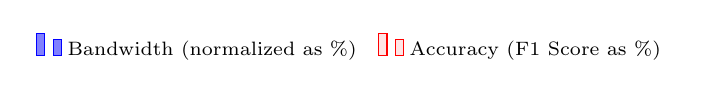
\begin{tikzpicture}
      \tikzstyle{every node}=[font=\scriptsize]
      \begin{axis}[
        width = 4cm,
        height = 2cm,
        hide axis,
        xmin=0,
        xmax=1,
        ymin=0,
        ymax=1,
        legend style={
          draw = none,
          legend columns= -1},
          /tikz/every even column/.append style={column sep=0.2cm},
        ]
        \addlegendimage{ybar, ybar legend, blue, fill=blue!50!white}\addlegendentry{B}
        \addlegendimage{ybar, ybar legend, red, fill=red!10!white}\addlegendentry{A}
        \legend{Bandwidth (normalized as \%), Accuracy (F1 Score as \%)}
      \end{axis}
    \end{tikzpicture}
  \end{minipage}
  \hfill
  \begin{minipage}{0.2\textwidth}
  \end{minipage}
  \\
  \vspace{0.1em}

  %%%
  %% First Half
  %%%

  \begin{subfigure}{0.07\textwidth}
    \footnotesize
    \centering
    \vspace{-2em}
    Stationary \\
    Camera
  \end{subfigure}%
  \begin{subfigure}{0.24\textwidth}
    \begin{tikzpicture}
      \tikzstyle{every node}=[font=\scriptsize]
      \begin{axis}[my bar,
        symbolic x coords = {30, 10, 5, 3, 2},
        ]

        \addplot [draw=blue, fill=blue!50!white, text=blue]
        table[x = Frame Rate, y = Bandwidth (normalized)]{\stationaryframerate};

        \addplot [draw=red, fill=red!10!white, text=red]
        table[x = Frame Rate, y = Accuracy]{\stationaryframerate};
        \legend{}
      \end{axis}
    \end{tikzpicture}
    \caption{Frame Rate \\ (resolution = 1080p)}
    \label{fig:stationary-frame-rate}
  \end{subfigure}%
  \begin{subfigure}{0.24\textwidth}
    \begin{tikzpicture}
      \tikzstyle{every node}=[font=\scriptsize]
      \begin{axis}[my bar,
        symbolic x coords = {1080p, 900p, 720p, 540p, 360p},
        ]
        \addplot [draw=blue, fill=blue!50!white, text=blue]
        table[x = Resolution, y = Bandwidth (normalized)]{\stationaryresolution};

        \addplot [draw=red, fill=red!10!white, text=red]
        table[x = Resolution, y = Accuracy]{\stationaryresolution};
        \legend{}
      \end{axis}
    \end{tikzpicture}
    \caption{Resolution \\ (frame rate = 30)}
    \label{fig:stationary-resolution}
  \end{subfigure}%
  \hspace{1em}
  \begin{subfigure}{0.2\textwidth}
    \includegraphics[width=\textwidth]{figures/mot-1.jpg}
    \caption{t = 0s \\ small targets in far-field views}
  \end{subfigure}
  \hspace{.2em}
  \begin{subfigure}{0.2\textwidth}
    \includegraphics[width=\textwidth]{figures/mot-2.jpg}
    \caption{t = 1s \\ small difference compared to t=0s}
  \end{subfigure}

  \vspace{0.7em}

  %%%%%%%%%%%%%%%%%%%%%%%%%%%%%%%%%%%%%%%%
  %% Second half
  %%%%%%%%%%%%%%%%%%%%%%%%%%%%%%%%%%%%%%%%

  \begin{subfigure}{0.07\textwidth}
    \footnotesize
    \centering
    \vspace{-3em}
    Mobile \\
    Camera
  \end{subfigure}%
  \begin{subfigure}{0.24\textwidth}
    \begin{tikzpicture}
      \tikzstyle{every node}=[font=\scriptsize]
      \begin{axis}[my bar,
        symbolic x coords = {30, 10, 5, 3, 2},
        ]
        \addplot [draw=blue, fill=blue!50!white, text=blue]
        table[x = Frame Rate, y = Bandwidth (normalized)]{\mobileframerate};

        \addplot [draw=red, fill=red!10!white, text=red]
        table[x = Frame Rate, y = Accuracy]{\mobileframerate};
        \legend{}
      \end{axis}
    \end{tikzpicture}
    \caption{Frame Rate \\ (resolution = 1080p)}
    \label{fig:mobile-frame-rate}
  \end{subfigure}%
  \begin{subfigure}{0.24\textwidth}
    \begin{tikzpicture}
      \tikzstyle{every node}=[font=\scriptsize]
      \begin{axis}[my bar,
        symbolic x coords = {1080p, 900p, 720p, 540p, 360p},
        ]
        \addplot [draw=blue, fill=blue!50!white, text=blue]
        table[x = Resolution, y = Bandwidth (normalized)]{\mobileresolution};

        \addplot [draw=red, fill=red!10!white, text=red]
        table[x = Resolution, y = Accuracy]{\mobileresolution};
        \legend{}
      \end{axis}
    \end{tikzpicture}
    \caption{Resolution \\ (frame rate = 30)}
    \label{fig:mobile-resolution}
  \end{subfigure}%
  \hspace{1em}
  \begin{subfigure}{0.2\textwidth}
    \includegraphics[width=\textwidth]{figures/darknet-1.jpg}
    \caption{t = 0s \\ nearby and large targets}
  \end{subfigure}
  \hspace{.2em}
  \begin{subfigure}{0.2\textwidth}
    \includegraphics[width=\textwidth]{figures/darknet-2.jpg}
    \caption{t = 1s \\ large difference compared to t=0s}
  \end{subfigure}

  \caption{The measured bandwidth and application accuracy for two video
    analytics applications. (1) Manual policies lack precision without
    measurements and need to handle multiple dimensions, as in (a-b) and
    (c-d). (2) Application-specific optimizations do not generalize: degrading
    frame rates works well for stationary camera (a), but not for mobile camera
    (e). (c-d) and (g-h) show example frames.}
  \label{fig:app-specific}
\end{figure*}

\captionsetup[subfigure]{
  font=small,
  skip=5pt,
}

%%% Local Variables:
%%% mode: latex
%%% TeX-master: "../awstream"
%%% End:
